\documentclass[twoside,final]{hcmut-report}

\usepackage[utf8]{inputenc}
\usepackage[T5]{fontenc}
\usepackage[vietnamese]{babel}
% \usepackage{vntex}
\usepackage[protrusion=false]{microtype}

\usepackage{graphicx, caption}
\usepackage{amsmath}
\usepackage{xcolor}
\usepackage{listings}
\usepackage{multirow,multicol}
\usepackage{enumitem}
\usepackage{hyperref}
\usepackage{float}
\usepackage{booktabs}
\usepackage{longtable}
\usepackage{array}
\usepackage{tabularx}
\usepackage{makecell}
\usepackage{subcaption}
\usepackage{tikz}
\usepackage{pgfplots}

\AtBeginDocument{\counterwithin{lstlisting}{section}}
\newcommand{\exercise}[1]{\noindent\begin{tikzpicture}
    \node[draw, rounded corners=3mm, text width=0.985\textwidth, align=justify]
    at (0,0){#1};
\end{tikzpicture}}

\begin{document}

\coverpage\clearpage
\tableofcontents
\clearpage

\fancyfoot{}
\fancyfoot[L]{\scriptsize \ttfamily Toán 12 - Ltro x doxncwfn - 2526}
\fancyfoot[R]{\scriptsize \ttfamily Trang {\thepage}/\pageref{LastPage}}

\setcounter{page}{1}
\section{Xác suất thống kê}
\subsection{Lý thuyết}
\subsection{Định nghĩa}
Cho hai biến cố $A$ và $B$. Xác suất của biến cố $A$ với điều kiện biến cố $B$ đã xảy ra được gọi là xác suất của $A$ với điều kiện $B$, kí hiệu là $P(A | B)$.

Nếu $P(B) > 0$ thì:
\[
    P(A | B) = \frac{P(A \cap B)}{P(B)}.
\]
\paragraph*{Nhận xét}
\begin{itemize}[itemsep=0pt, topsep=0pt, parsep=0pt,label=-]
    \item Từ định nghĩa của xác suất có điều kiện, ta suy ra $P(A \cap B) = P(B) \cdot P(A | B)$.
    \item Người ta chứng minh được rằng
          \[
              \mathrm{P}(A \cap B) = \mathrm{P}(A) \cdot \mathrm{P}(B | A) = \mathrm{P}(B) \cdot \mathrm{P}(A | B).
          \]
          Công thức trên được gọi là \textbf{công thức nhân xác suất}.
    \item Người ta cũng tính $P(A | B) = \dfrac{n(A \cap B)}{n(B)}$.
\end{itemize}
\subsubsection{Công thức xác suất đầy đủ}
Cho 2 biến cố $A$, $B$ với $0 < P(B) < 1$, ta có:
\[
    P(A) = P(A \cap B) + P(A \cap \overline{B}).
\]

Mặt khác:
\begin{align*}
    P(A \cap B)            & = P(B) \cdot P(A | B)                       \\
    P(A \cap \overline{B}) & = P(\overline{B}) \cdot P(A | \overline{B})
\end{align*}

Từ đó ta có công thức xác suất đầy đủ như sau:
\[
    P(A) = P(B) \cdot P(A | B) + P(\overline{B}) \cdot P(A | \overline{B}).
\]
\subsubsection{Công thức Bayes}
Từ công thức nhân xác suất:
\[
    P(B | A) \cdot P(A) = P(B) \cdot P(A | B) = P(A \cap B).
\]

Với hai biến cố $A, B$ mà $P(A) > 0$, ta có công thức xác suất Bayes:
\[
    P(B | A) = \frac{P(B) \cdot P(A | B)}{P(A)}.
\]

Do \(P(A) = P(B) \cdot P(A | B) + P(\overline{B}) \cdot P(A | \overline{B})\), nên công thức Bayes còn có dạng:
\[
    P(B | A) = \frac{P(B) \cdot P(A | B)}{P(B) \cdot P(A | B) + P(\overline{B}) \cdot P(A | \overline{B})}.
\]
\subsection{Bài tập}
\exercise{Theo một số liệu thống kê, năm 2004 ở Canada có 65\% nam giới là thừa cân và 53,4\% nữ giới là thừa cân. Nam giới và nữ giới ở Canada đều chiếm 50\% dân số cả nước. Hỏi trong năm 2004, xác suất để một người Canada được chọn ngẫu nhiên là người thừa cân bằng bao nhiêu?}

Xét hai biến cố:
\begin{itemize}[itemsep=0pt, topsep=0pt, parsep=0pt,label=-]
    \item $A$: ``Người được chọn ra là người thừa cân'';
    \item $B$: ``Người được chọn ra là nam giới'' $\Rightarrow\overline{B}$: ``Người được chọn ra là nữ giới''.
\end{itemize}

Từ giả thiết:
$\begin{cases}
        \mathrm{P}(B) = \mathrm{P}(\overline{B}) = 50\% = 0{,}5 \\
        \mathrm{P}(A | B) = 65\% = 0{,}65                       \\
        \mathrm{P}(A | \overline{B}) = 53{,}4\% = 0{,}534.
    \end{cases}$

Theo công thức xác suất toàn phần:
\[
    \mathrm{P}(A) = \mathrm{P}(B) \cdot \mathrm{P}(A | B) + \mathrm{P}(\overline{B}) \cdot \mathrm{P}(A | \overline{B})
    = 0{,}5 \cdot 0{,}65 + 0{,}5 \cdot 0{,}534 = 0{,}592.
\]
\subsection{Đề thi thử trường sở}
\exercise{
    \hspace*{0.5cm} \textcolor{orange}{\textit{Đợt 3 -- 2425 -- Nghệ An}}\\
    \hspace*{0.5cm} Một nghiên cứu dịch tễ học trong một cộng đồng dân số tại một địa phương X đưa ra các số liệu sau:
    \begin{itemize}[itemsep=0pt, topsep=0pt, parsep=0pt,label=-]
        \item Tỷ lệ người có hút thuốc lá là 25\%.
        \item Tỷ lệ bị ung thư phổi ở nhóm người hút thuốc lá là 2\%, trong khi ở nhóm người không hút thuốc lá chỉ là 0,1\%.
    \end{itemize}

    \hspace*{0.5cm} Xét một người được chọn ngẫu nhiên từ cộng đồng này. Ký hiệu $A$ là biến cố "Người đó bị ung thư phổi" và $B$ là biến cố "Người đó có hút thuốc lá".

    \begin{enumerate}[itemsep=0pt, topsep=0pt, parsep=0pt,label=\alph*)]
        \item $P(A|B) = 0,1$
        \item Nếu một người bị ung thư phổi, thì xác suất người đó có hút thuốc lá là 0,8 (làm tròn đến hàng phần mười).
        \item Tỷ lệ người bị ung thư phổi ở địa phương X là 1,5\%
        \item Dựa trên các số liệu này, tỷ lệ người bị ung thư phổi ở nhóm người có hút thuốc lá cao gấp 20 lần so với ở nhóm người không hút thuốc.
    \end{enumerate}}

\begin{minipage}{0.45\textwidth}
    \begin{figure}[H]
        \centering
        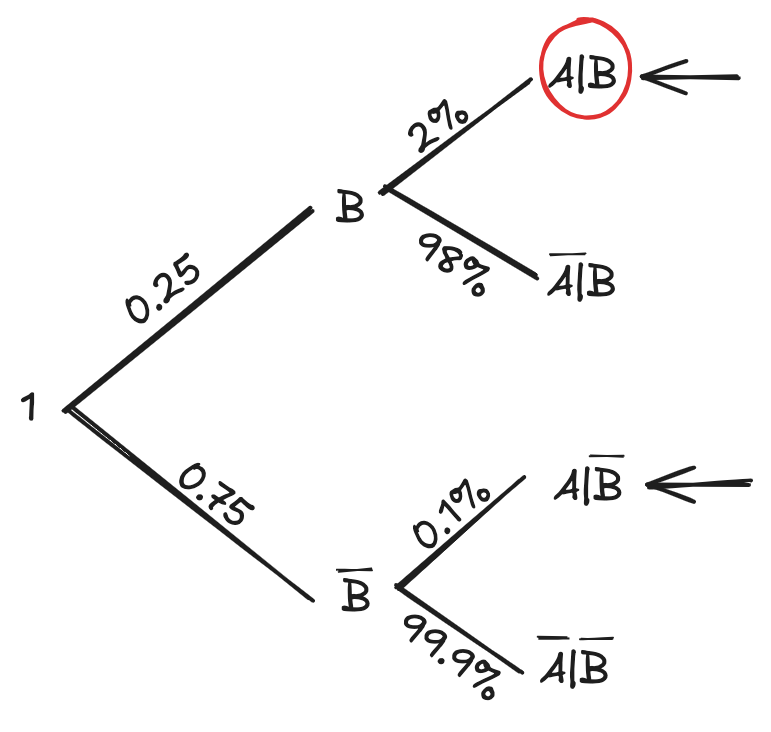
\includegraphics[width=\textwidth]{images/1.4.1.png}
    \end{figure}
\end{minipage}
\begin{minipage}{0.55\textwidth}
    a) Từ đề bài: $\begin{cases}
            P(A|B)=2\%                \\
            P(A|\overline{B}) = 0,1\% \\
            P(B) = 0.25
        \end{cases} \Rightarrow$ \textcolor{red}{Sai}

    b) $P(A|B) = \dfrac{2\%\cdot 0.25}{2\%\cdot 0.25 + 0.75\cdot 0.1\%} = \dfrac{20}{23} \approx 0.9 \Rightarrow$ \textcolor{red}{Sai}

    c) $P(A) = 2\%\cdot 0.25 + 0.1\%\cdot 0.75 = 5.75\%\Rightarrow$ \textcolor{red}{Sai}

    d) $\dfrac{P(A|B)}{P(A|\overline{B})} = \dfrac{2\%}{0.1\%} = 20\Rightarrow$  \textcolor{red}{Đúng}
\end{minipage}
\end{document}